\chapter{نمونه اولیه واسط کاربری}
در این فصل تصاویری از ویژگی‌های طراحی شده در نمونه اولیه واسط کاربری تکرار دوم فاز تفصیل به‌تفکیک زیرسیستم نیازمندی‌های مربوطه ارائه می‌شود.
\section{تصاویر ویژگی‌های زیرسیستم‌ها}
در این بخش 14 نیازمندی جهت نمایش انتخاب شده که نمونه اولیه واسط کاربری را از دید زیرسیستم‌ها نمایش دهد.
برای طراحی صفحات واسط کاربری سیستم از کتابخانه \lr{React} و زبان \lr{TypeScript} بهره گرفته شده است.

ترتیب ارائه‌ی نیازمندی‌ها به‌گونه‌ای انتخاب شده که درک نقشه سامانه واسط کاربری آسان گردد. در ابتدا صفحه‌ی اصلی سایت که در حال حاضر صرفاً شامل دکمه ثبت‌نام/ورود است مطابق شکل \ref{homepage} طراحی اولیه شده است:

\begin{figure}[h]
	\centering
	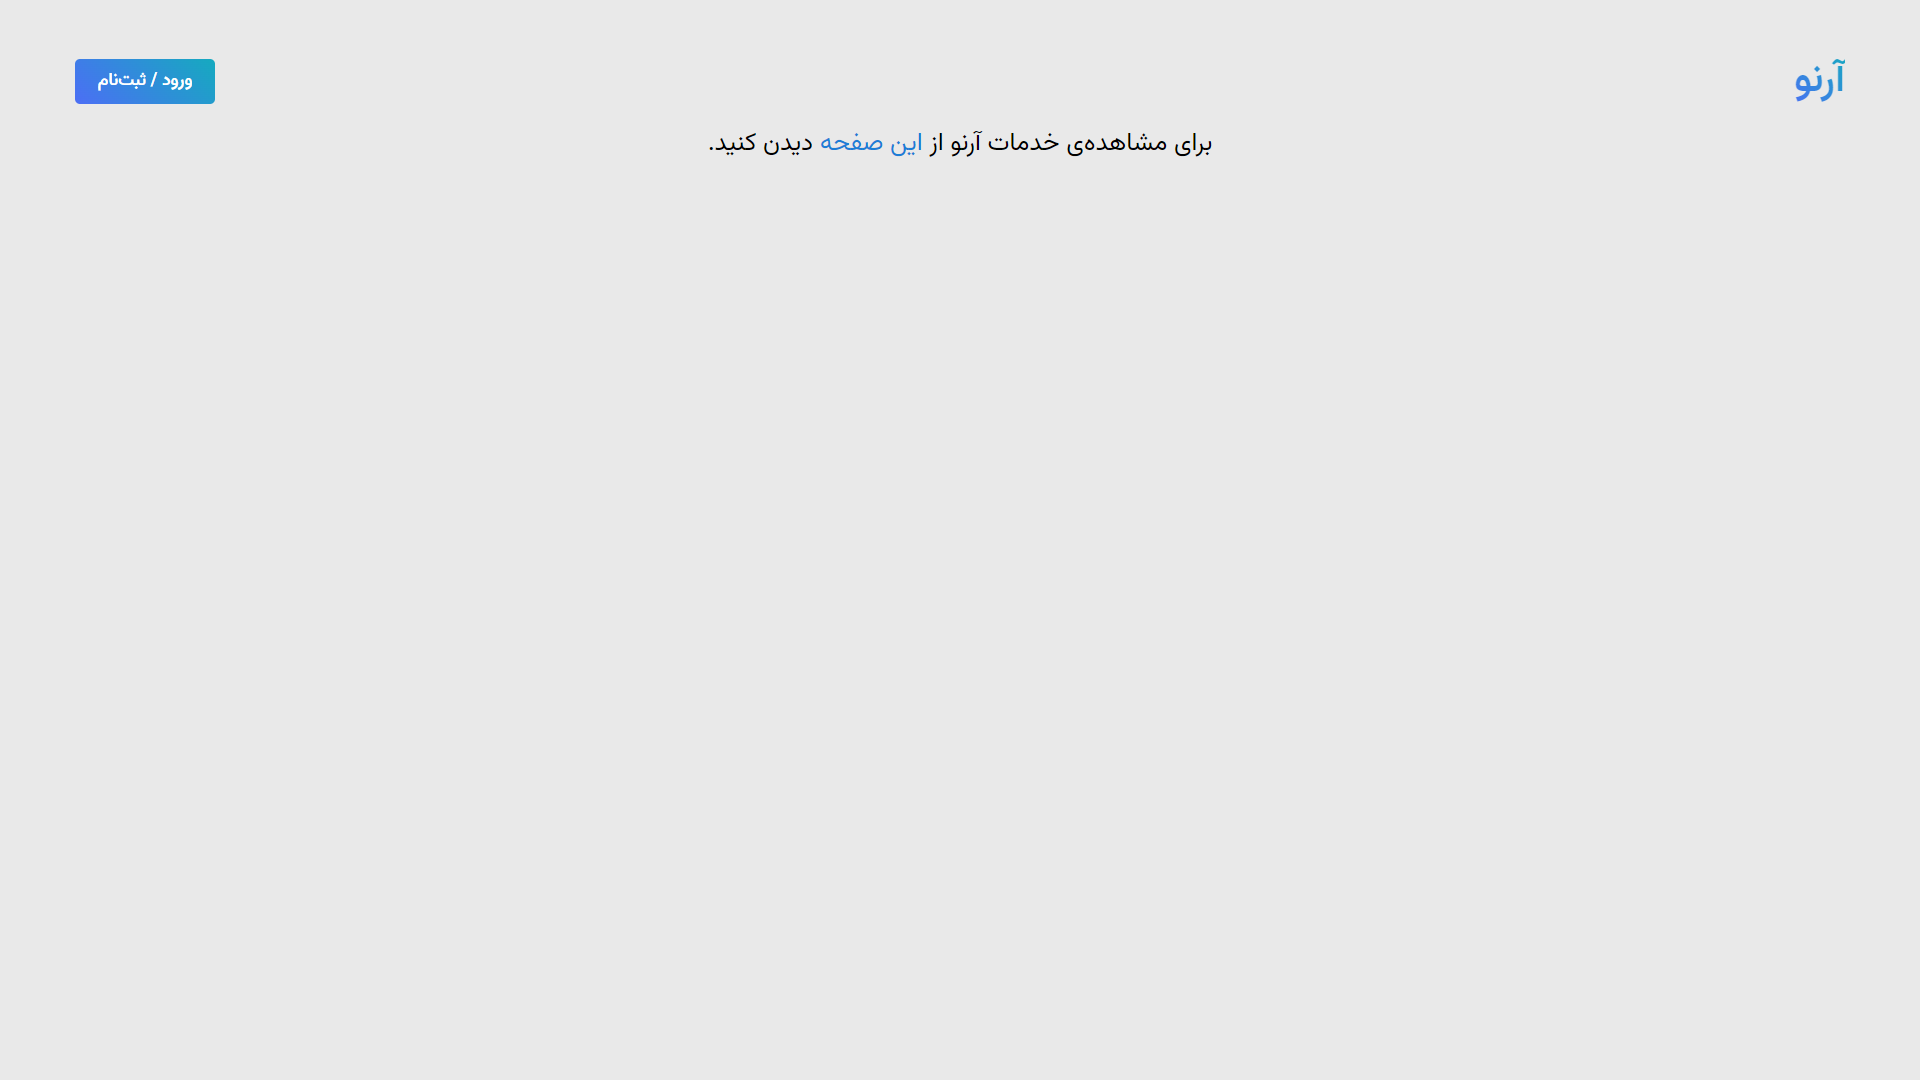
\includegraphics[width=\textwidth]{figs/initial-ui/homepage}
	\caption{صفحه اصلی}
	\label{homepage}
\end{figure}

\subsection{زیرسیستم کاربری}

\subsubsection{‌ثبت‌نام و ویرایش اطلاعات کاربری}
شکل
\ref{req-15}
نمایانگر این ویژگی (شماره 15) است. در شکل
\ref{signup}
فرم ثبت نام و در شکل
\ref{edit-profile}

صفحه ویرایش پروفایل نمایش داده شده است. در این شکل در صورت ورود متخصص امکان فعال/غیرفعال کردن حساب نیز در فرم قرار گرفته است.

\begin{figure*}[h]
	\centering
	\begin{subfigure}[b]{\textwidth}
		\centering
		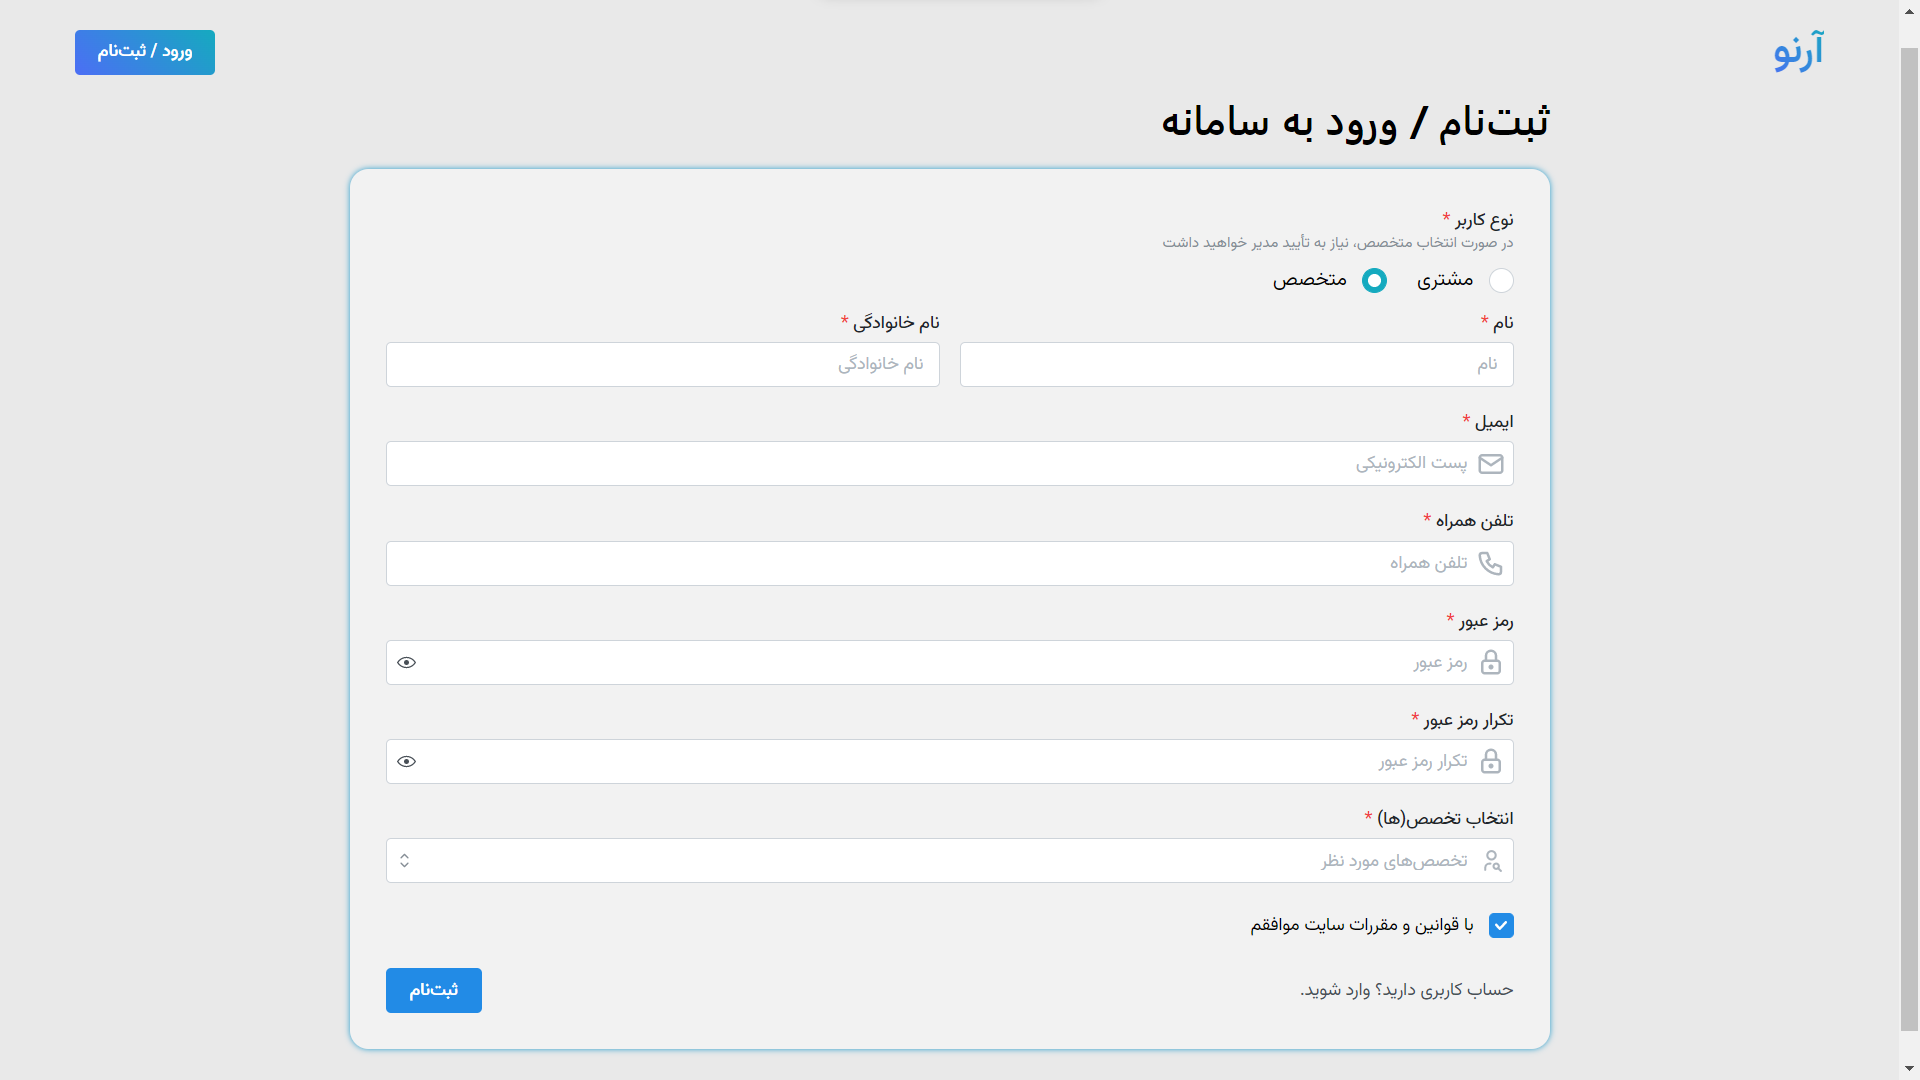
\includegraphics[width=\textwidth]{figs/initial-ui/signup}
		\caption[صفحه ثبت‌نام: در این قسمت در صورت انتخاب «متخصص» فیلد «انتخاب تخصص(ها)» نمایان می‌شود.]%
		{{\small صفحه ثبت‌نام: در این قسمت در صورت انتخاب «متخصص» فیلد «انتخاب تخصص(ها)» نمایان می‌شود.}}    
		\label{signup}
	\end{subfigure}
	\begin{subfigure}[b]{\textwidth}   
		\centering 
		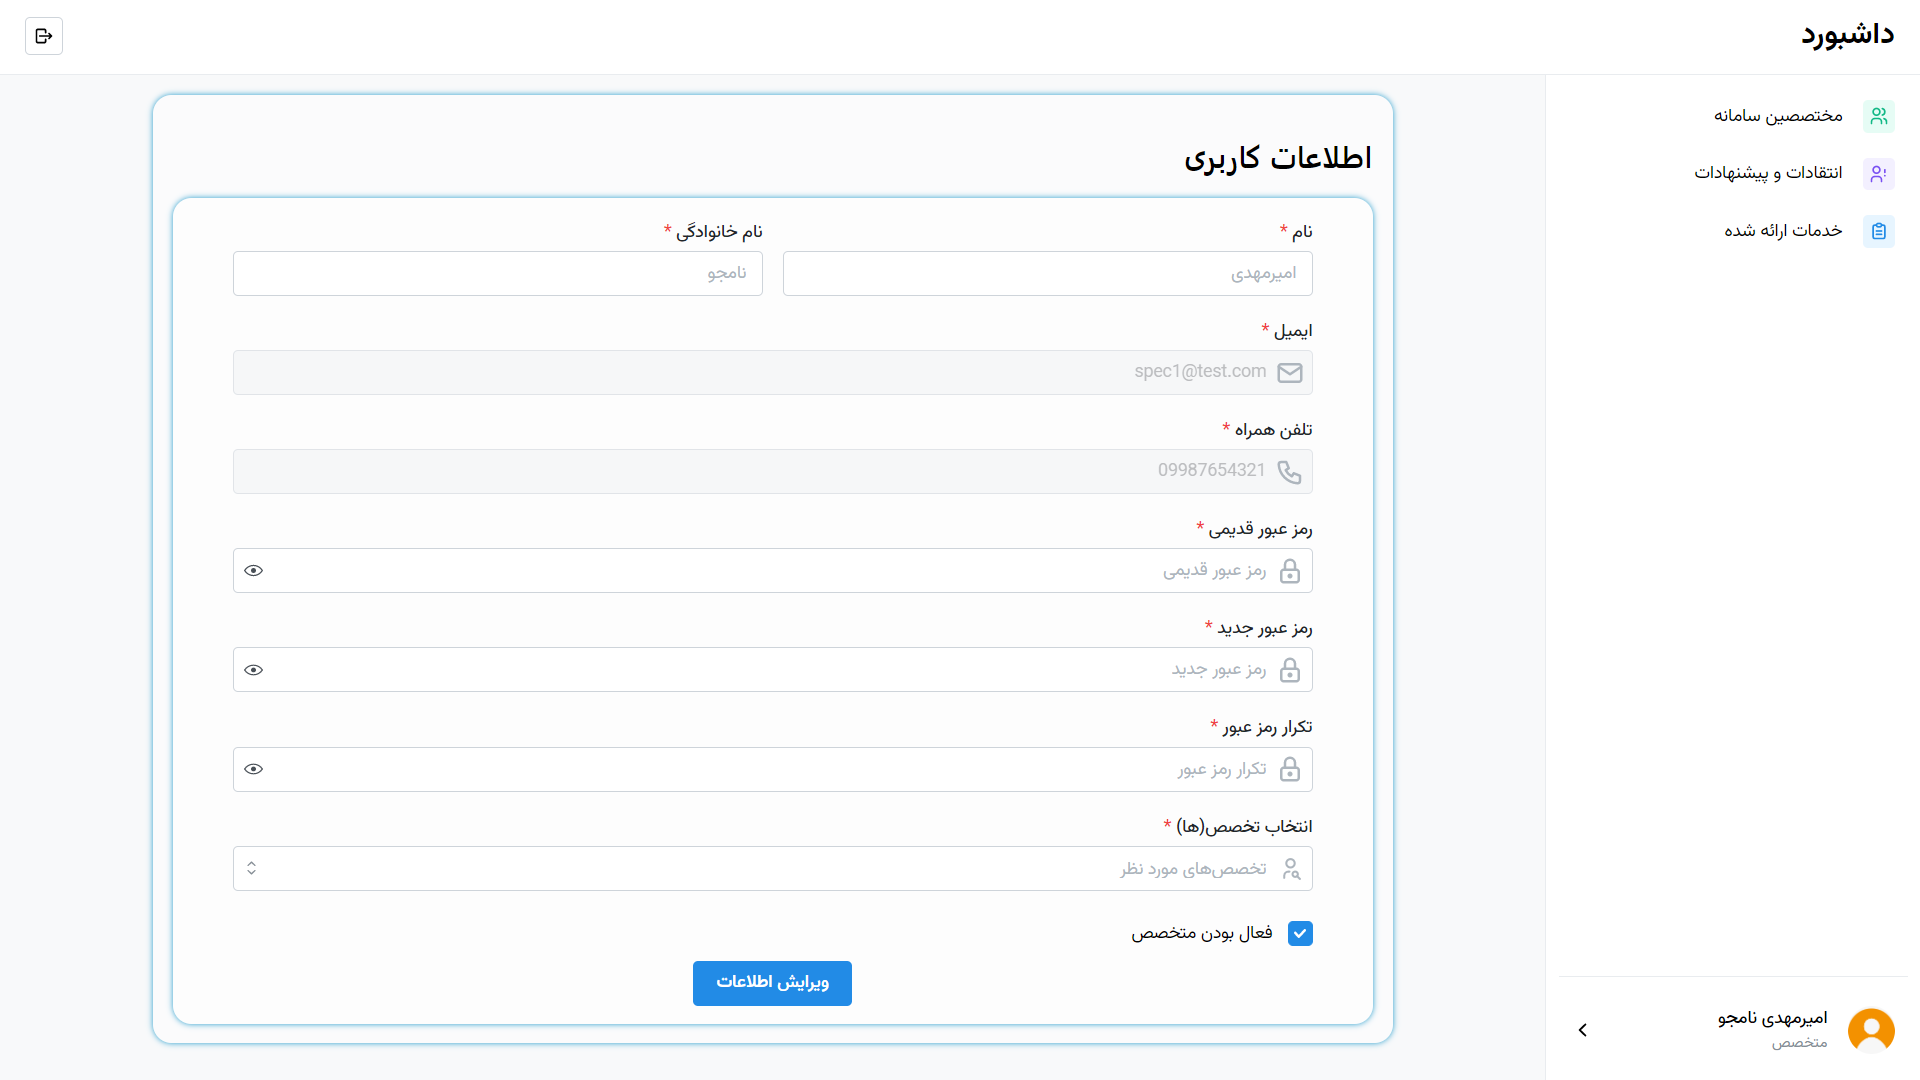
\includegraphics[width=\textwidth]{figs/initial-ui/edit-profile}
		\caption[ویرایش اطلاعات: این صفحه (قابل دسترسی از پایین داشبورد) به کاربران مختلف امکان ویرایش اطلاعات مربوط به نوع کاربری خود را می‌دهد.]%
		{{\small ویرایش اطلاعات: این صفحه (قابل دسترسی از پایین داشبورد) به کاربران مختلف امکان ویرایش اطلاعات مربوط به نوع کاربری خود را می‌دهد.}}    
		\label{edit-profile}
	\end{subfigure}
	\caption[ثبت‌نام و ویرایش پروفایل]
	{\small ثبت‌نام و ویرایش پروفایل} 
	\label{req-15}
\end{figure*}

\subsubsection{مشاهده لیست متخصصین براساس امتیاز}
این ویژگی (شماره 3) در شکل
\ref{spec-specialists}
به تصویر کشیده شده است. همانطور که مشاهده می‌شود متخصصین به‌ترتیب نزولی میانگین امتیاز مرتب شده‌اند.

\begin{figure}[h]
	\centering
	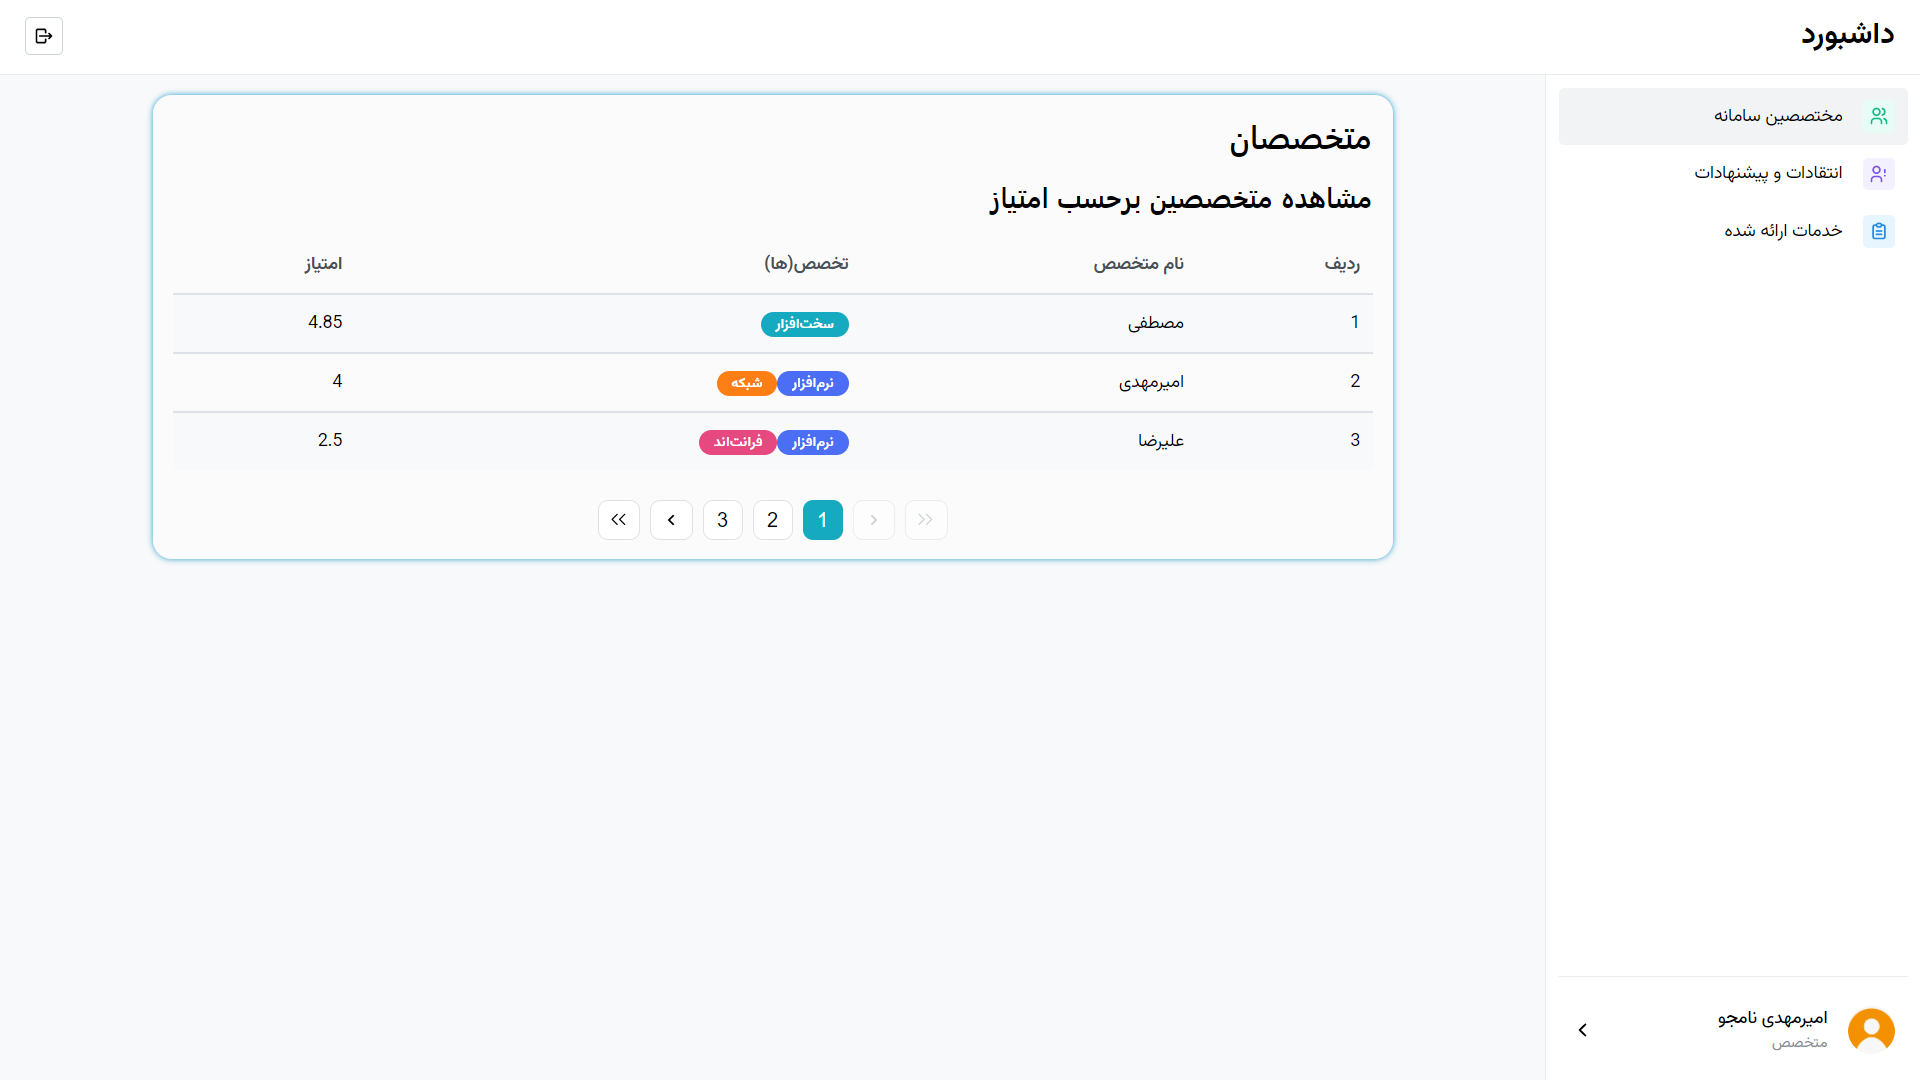
\includegraphics[width=\textwidth]{figs/initial-ui/spec-specialists}
	\caption{مشاهده متخصصین (قابل دسترسی برای همه کاربران)}
	\label{spec-specialists}
\end{figure}

\subsubsection{جست‌وجو در لیست متخصصین}
این ویژگی (شماره 11) در شکل
\ref{ctmr-specialists}
ترسیم شده است. همانطور که مشاهده می‌شود مشتریان می‌توانند علاوه بر مشاهده لیست متخصصین (که در قسمت قبل نشان داده شده) براساس تخصص‌ها و نام متخصص(های) مدنظر خود را بیابند.

\begin{figure}[h]
	\centering
	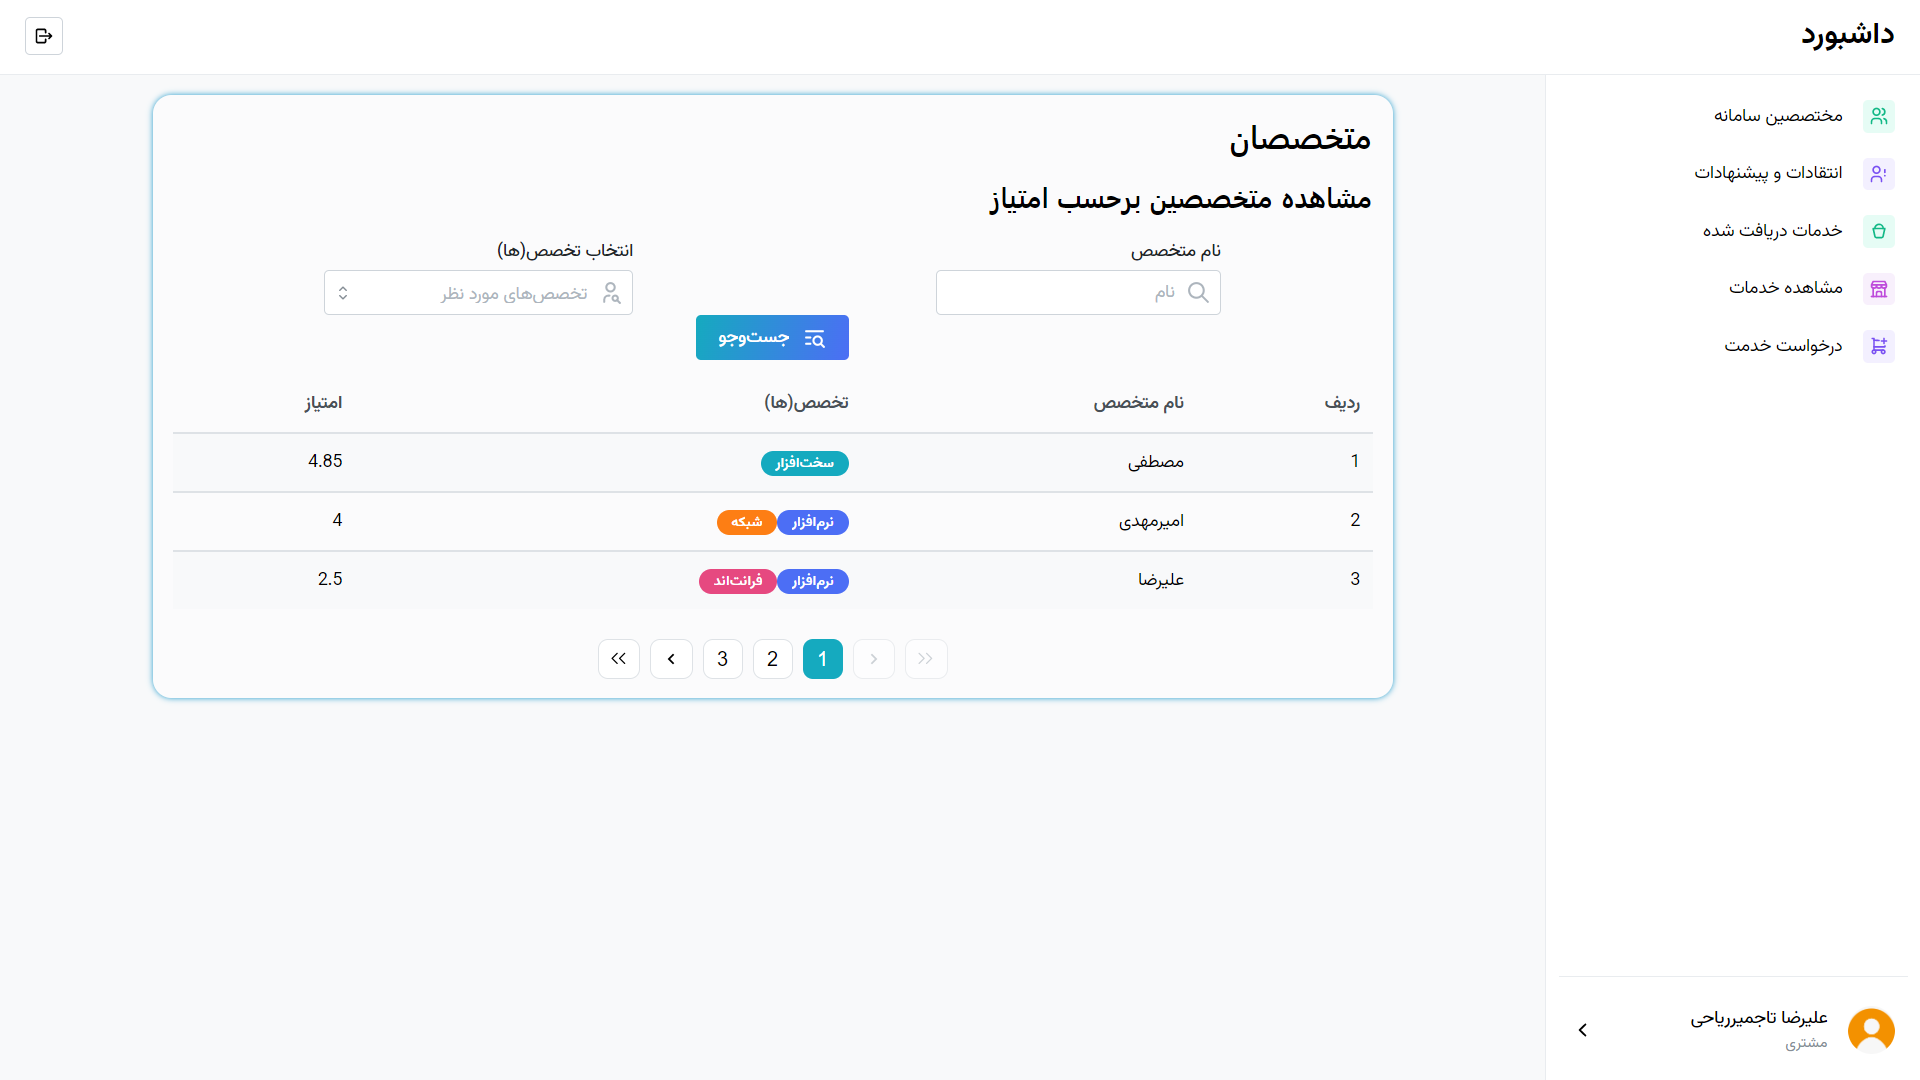
\includegraphics[width=\textwidth]{figs/initial-ui/ctmr-specialists}
	\caption{مشاهده متخصصین (قسمت جست‌وجو فقط برای مشتریان)}
	\label{ctmr-specialists}
\end{figure}


\subsection{زیرسیستم خدمت‌دهی}

\subsubsection{جست‌وجو و مشاهده خدمات}

در شکل
\ref{ctmr-services}
ویژگی جست‌وجو و مشاهده خدمات دسته‌بندی شده (شماره 10) نمایش داده شده است. این قابلیت تنها برای مشتریان وجود دارد.

\begin{figure}[h]
	\centering
	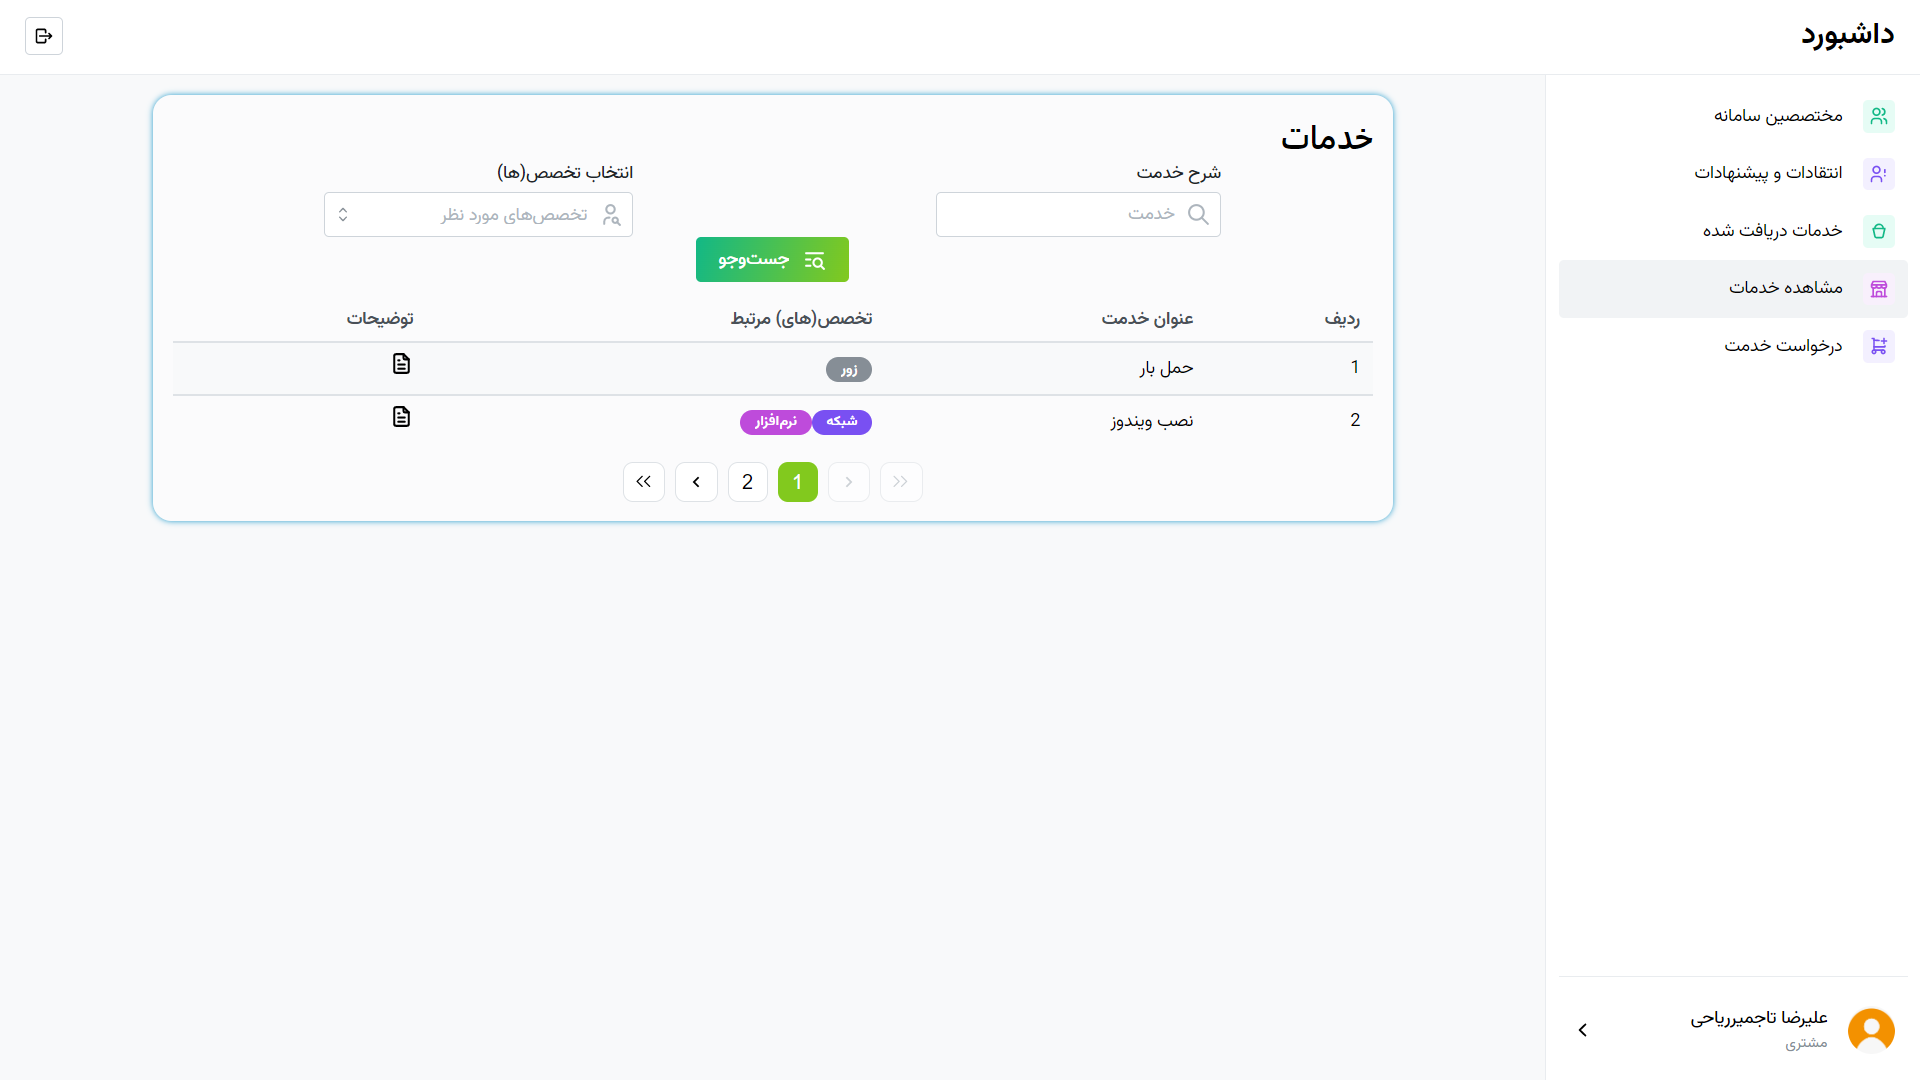
\includegraphics[width=\textwidth]{figs/initial-ui/ctmr-services}
	\caption{مشاهده و جست‌وجو در خدمات}
	\label{ctmr-services}
\end{figure}

\subsubsection{دو ویژگی رد متخصص و مشاهده وضعیت درخواست‌ها}
ویژگی‌های ذکر شده (شماره 12 و 24) در صفحه‌ی «سفارش‌های من» در پنل مشتری قرار گرفته‌اند که در شکل
\ref{ctmr-requests-spec}
نمایش داده شده است.

\begin{figure}[h]
	\centering
	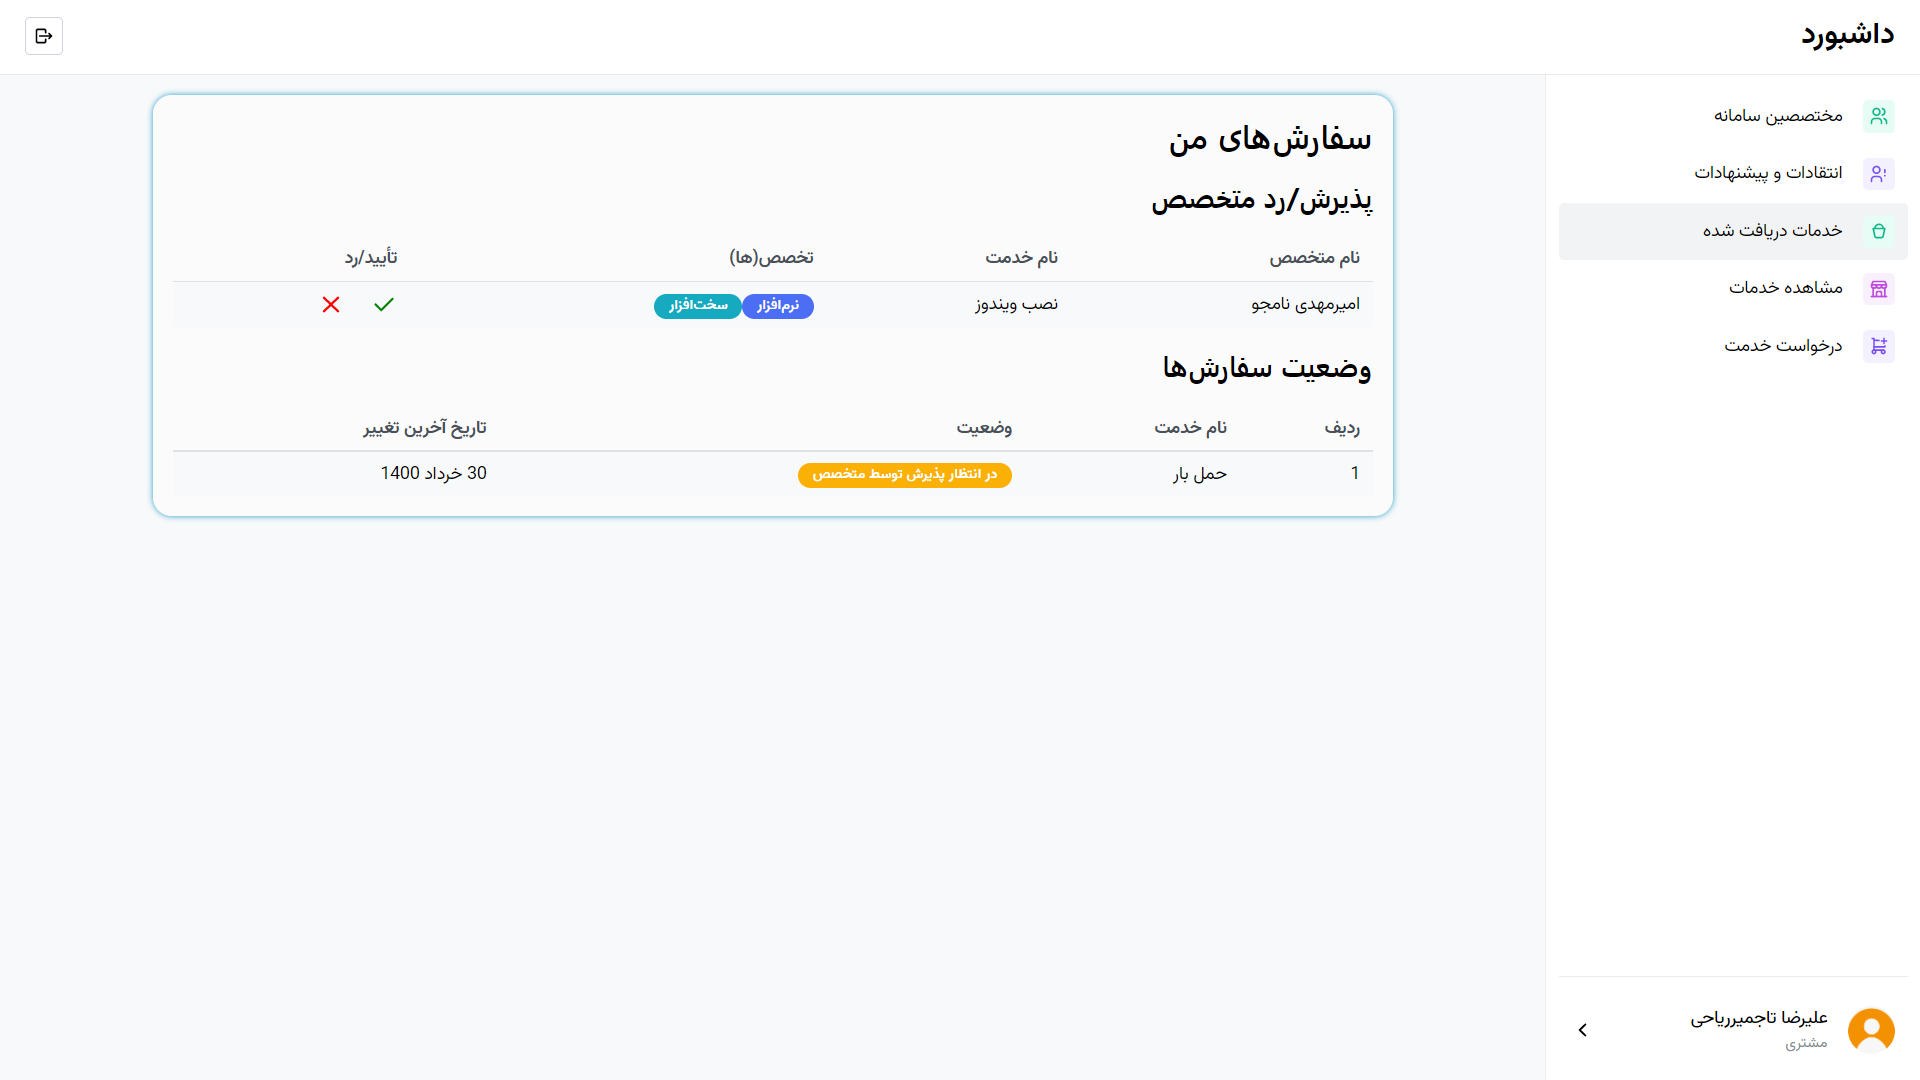
\includegraphics[width=\textwidth]{figs/initial-ui/ctmr-requests-spec}
	\caption{رد متخصص و نمایش وضعیت درخواست‌های مشتری}
	\label{ctmr-requests-spec}
\end{figure}

\subsubsection{دو ویژگی رد درخواست مشتری و دریافت پیام}
ویژگی‌های ذکر شده (شماره 13 و 14) در صفحه‌ی «خدمات ارائه شده» در پنل متخصص در شکل
\ref{spec-request-notif}
نشان داده شده‌اند (اعلان به متخصص در پایین چپ صفحه ظاهر می‌شود).

\begin{figure}[h]
	\centering
	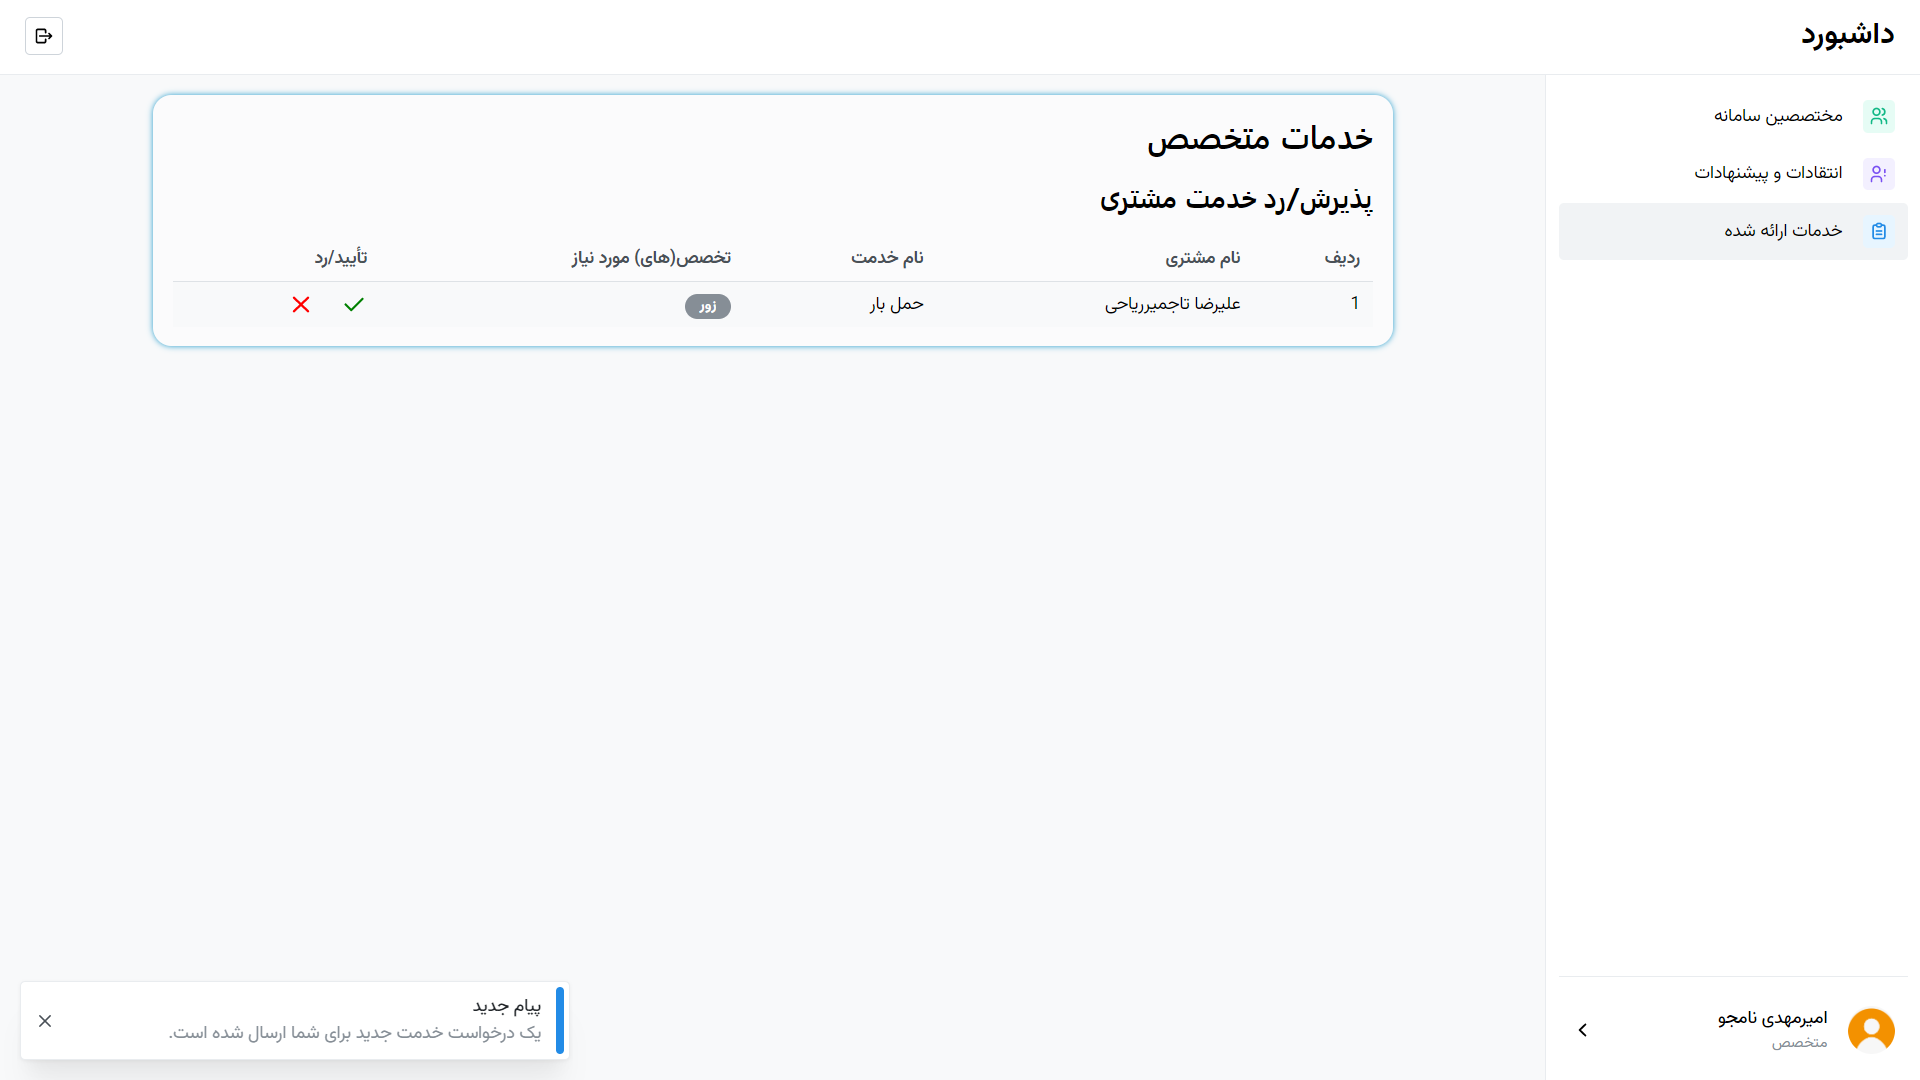
\includegraphics[width=\textwidth]{figs/initial-ui/spec-request-notif}
	\caption{پذیرش/رد مشتری توسط متخصص و دریافت اعلان}
	\label{spec-request-notif}
\end{figure}

\subsection{زیرسیستم گزارش‌گیری}

\subsubsection{دریافت گزارش مشکلات فنی}
شکل
\ref{mngr-tech-report}
ویژگی شماره 1 یعنی دریافت گزارش مشکلات فنی توسط مدیران را نشان می‌دهد. همچنین در شکل امکان مشاهده پاسخ مدیر فنی برای مدیر شرکت (ویژگی شماره 2) هم وجود دارد که در بخش مربوطه به آن پرداخته شده است.

\begin{figure}[h]
	\centering
	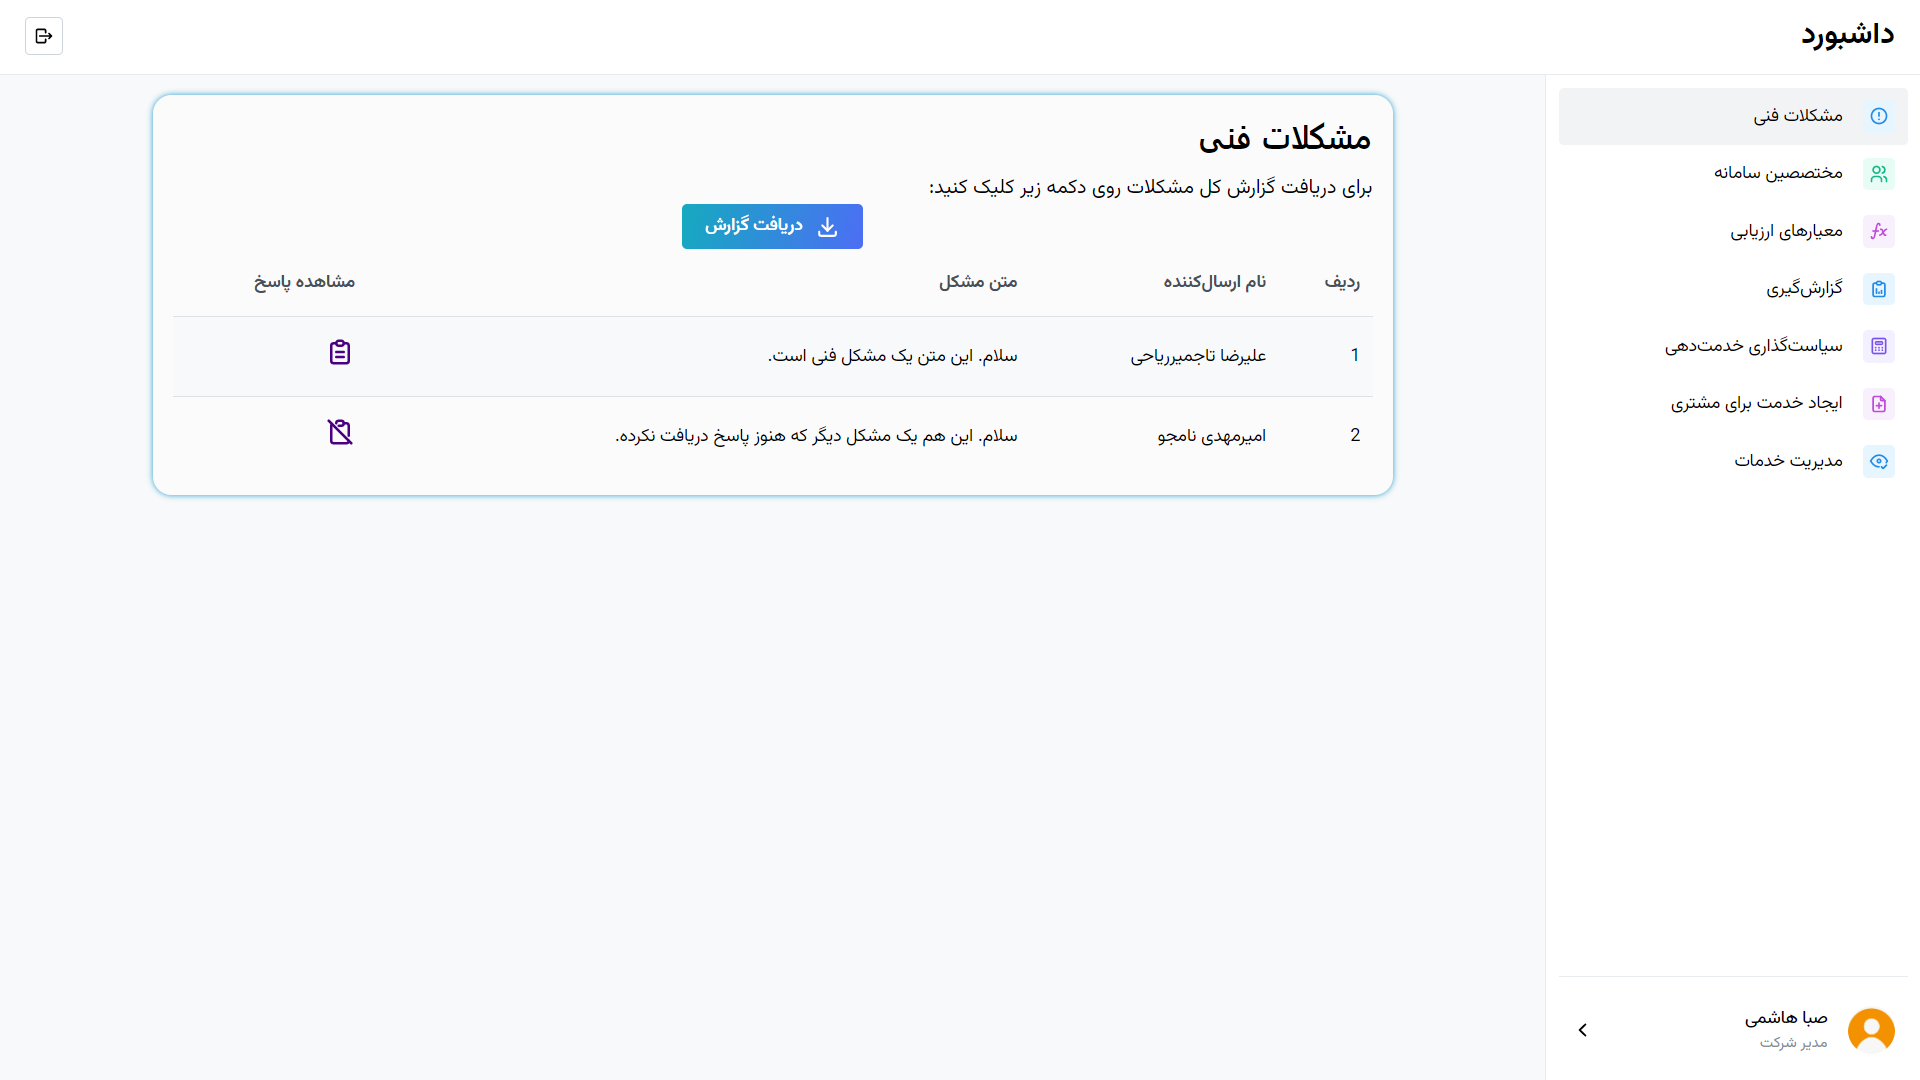
\includegraphics[width=\textwidth]{figs/initial-ui/mngr-tech-report}
	\caption{مشکلات فنی در پنل مدیر شرکت}
	\label{mngr-tech-report}
\end{figure}


\subsubsection{ارسال پاسخ به مشکلات فنی}
شکل
\ref{tech-tech-report}
ویژگی شماره 2 را نشان می‌دهد که طی آن مدیر فنی امکان مشاهده و ارسال پاسخ به مشکلات فنی کاربران را (با کلیک روی ستون سمت چپ جدول و نوشتن متن در یک \lr{Modal}) دارد. همانطور که در شکل
\ref{mngr-tech-report}
نشان داده شد، مدیر امکان مشاهده این پاسخ را خواهد داشت.

\begin{figure}[h]
	\centering
	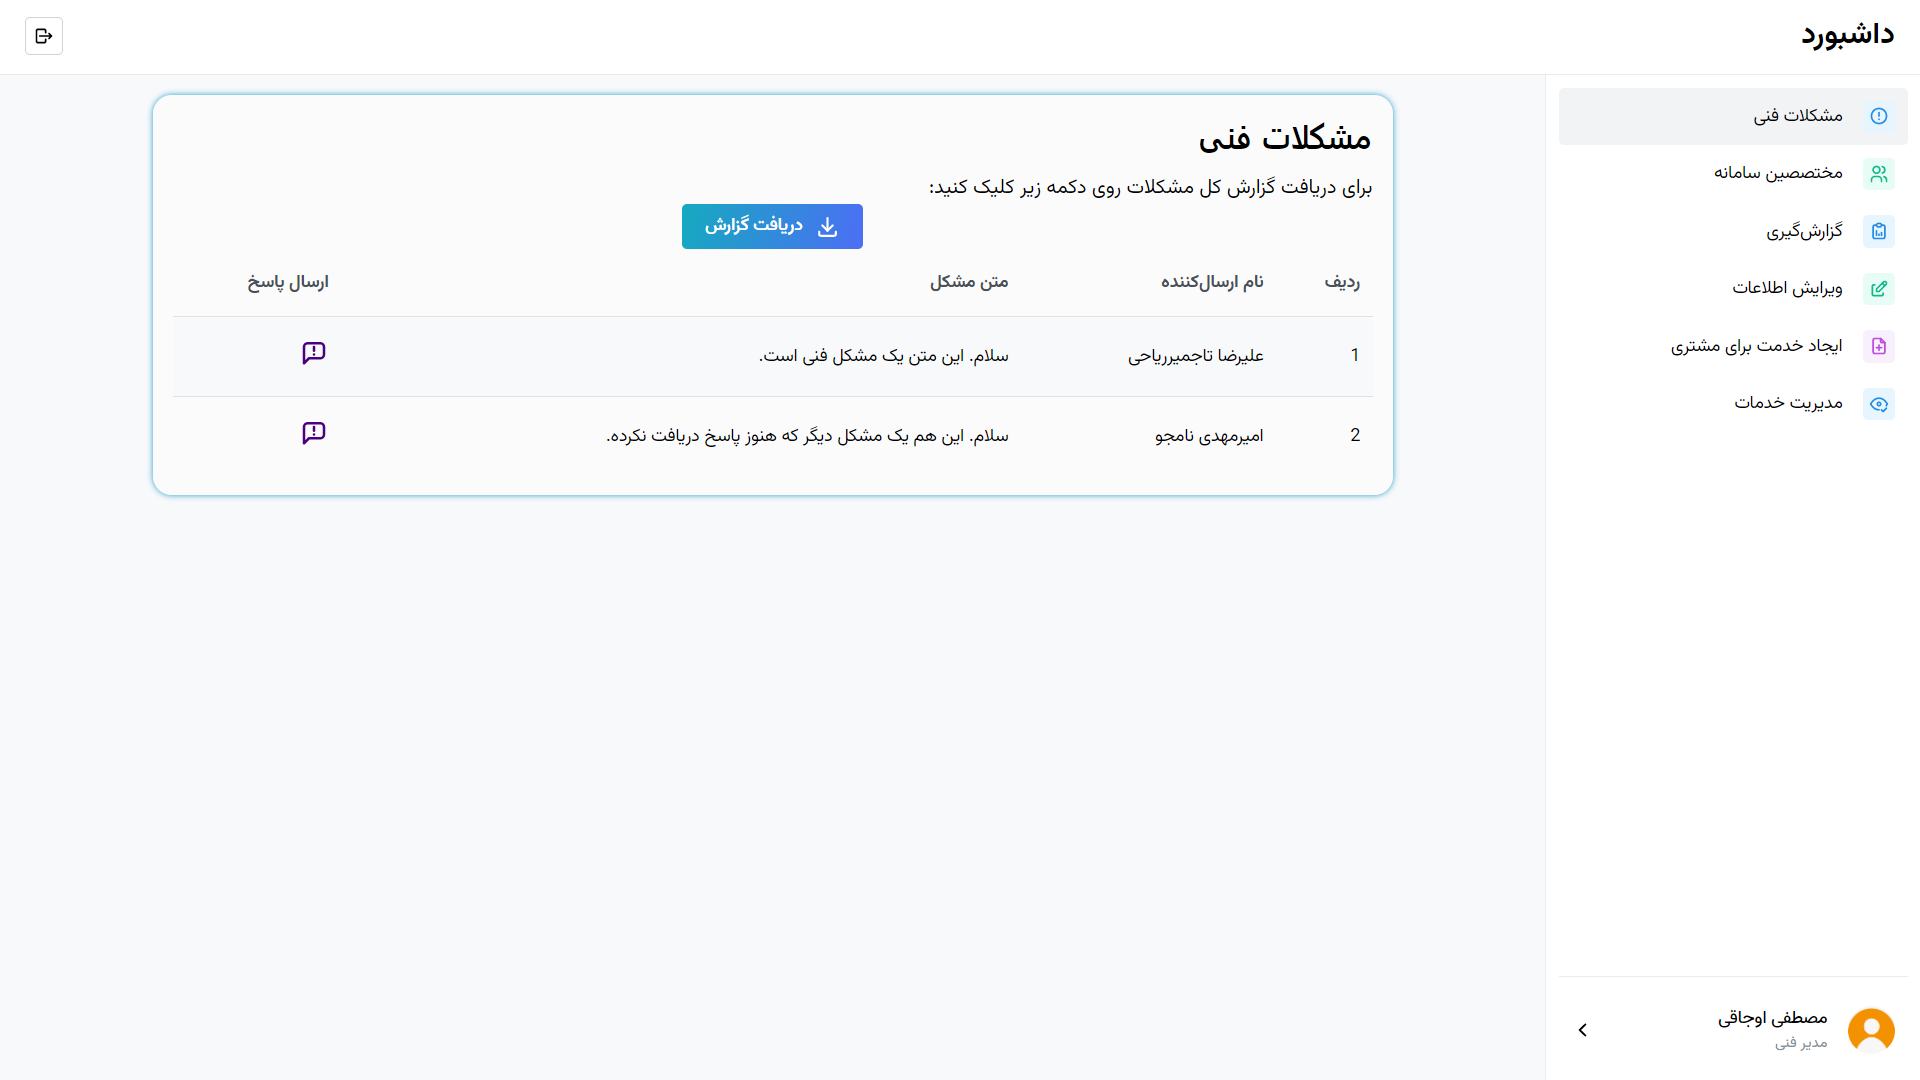
\includegraphics[width=\textwidth]{figs/initial-ui/tech-tech-report}
	\caption{مشکلات فنی در پنل مدیر فنی}
	\label{tech-tech-report}
\end{figure}

\subsection{زیرسیستم بازخورد}

\subsubsection{ثبت انتقادات، پیشنهادات و مشکلات فنی}
این ویژگی (شماره 5) در داشبورد متخصصین و مشتریان مطابق شکل
\ref{suggestions}
قرار گرفته و امکان ارسال انتقادات، پیشنهادات و مشکلات فنی را با ذکر نوع پیام فراهم می‌کند.

\begin{figure}[h]
	\centering
	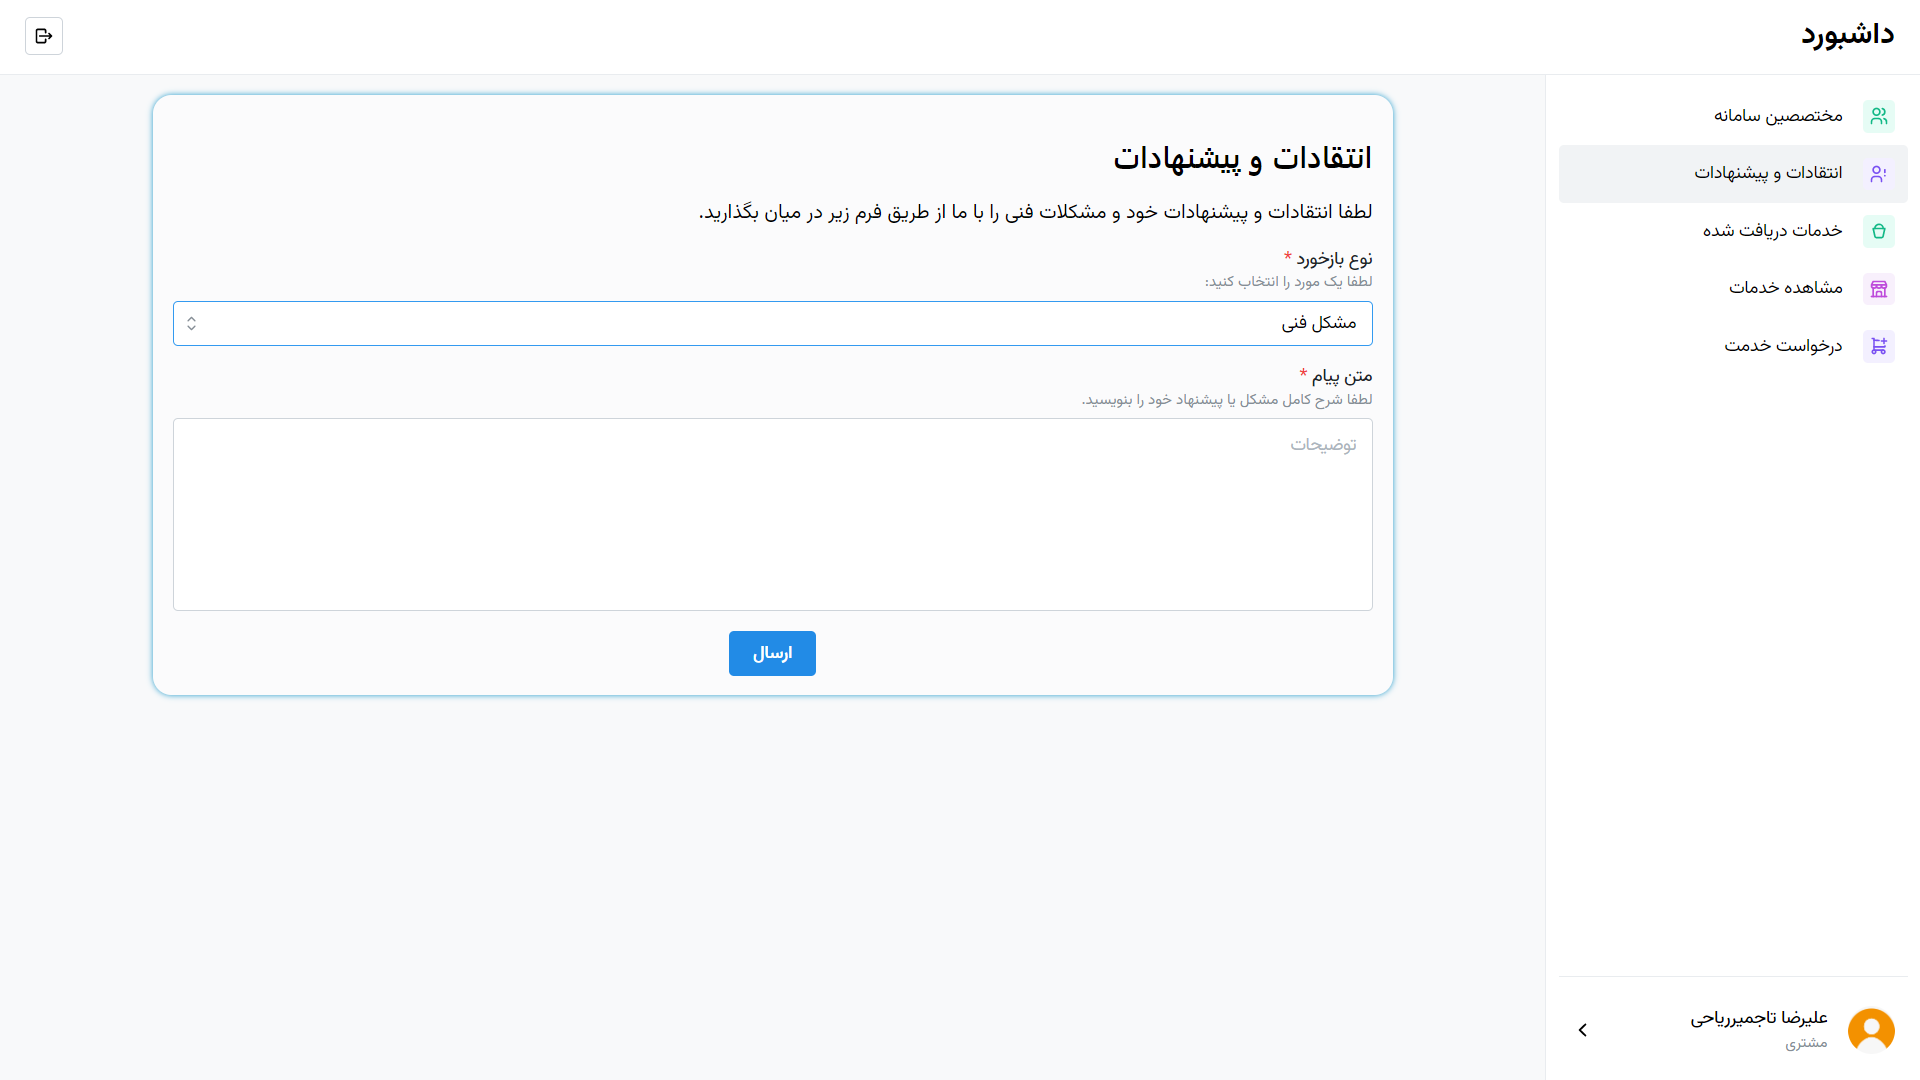
\includegraphics[width=\textwidth]{figs/initial-ui/suggestions}
	\caption{انتقادات، پیشنهادات و مشکلات فنی}
	\label{suggestions}
\end{figure}

\subsection{زیرسیستم مدیریت}

\subsubsection{تعیین سقف تعداد خدمات بر اساس امتیاز}
این ویژگی (شماره 9) که برای مدیر شرکت فراهم است در تصویر
\ref{policy}
نمایش داده شده است.

\begin{figure}[h]
	\centering
	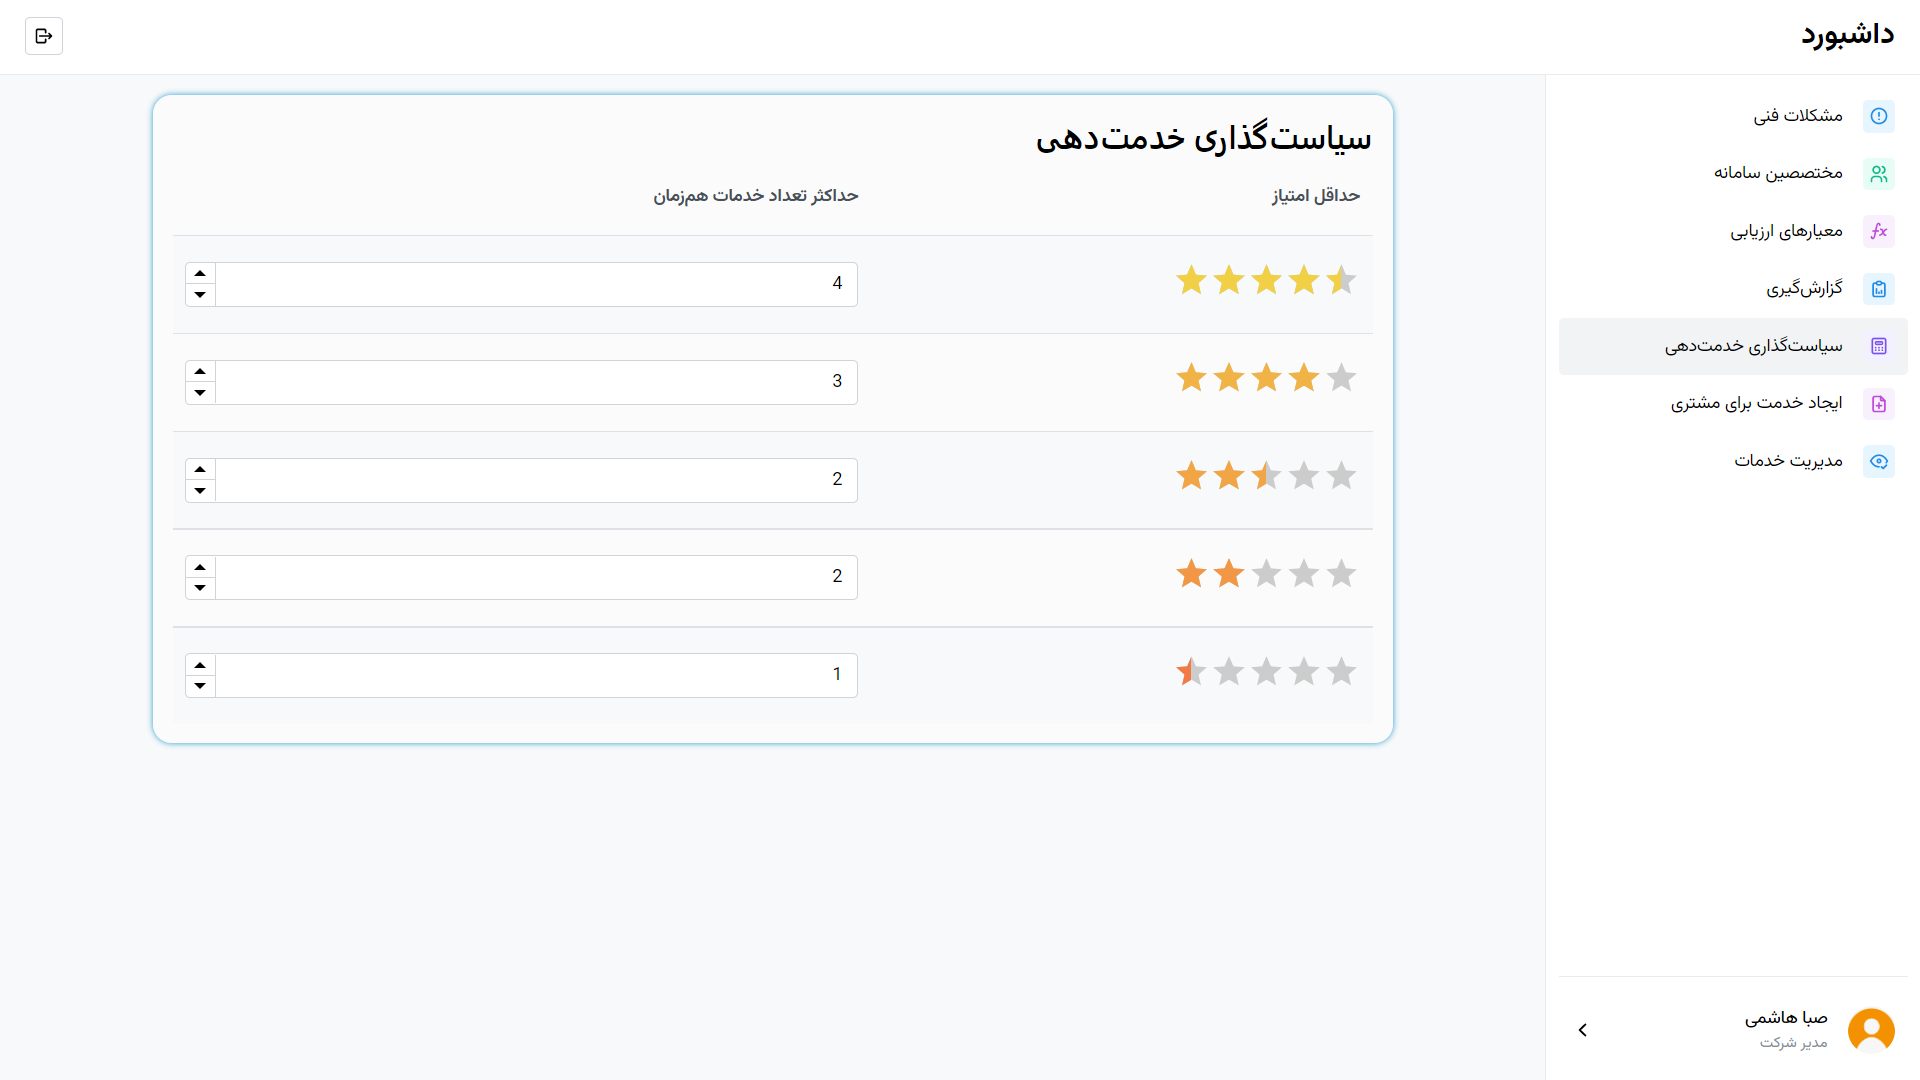
\includegraphics[width=\textwidth]{figs/initial-ui/service-policy}
	\caption{سیاست‌گذاری سقف تعداد خدمات متخصصین}
	\label{policy}
\end{figure}


\subsubsection{امکان تأیید متخصصین}
این ویژگی (شماره 18) در بالای شکل
\ref{mngr-specialists}
نشان داده شده است. قسمت دوم این شکل همان ویژگی شماره 3 (مشاهده لیست براساس امتیاز) را نشان می‌دهد که در شکل
\ref{ctmr-specialists}
بالاتر برای نوع کاربر غیر مدیر معرفی کردیم.

\begin{figure}[h]
	\centering
	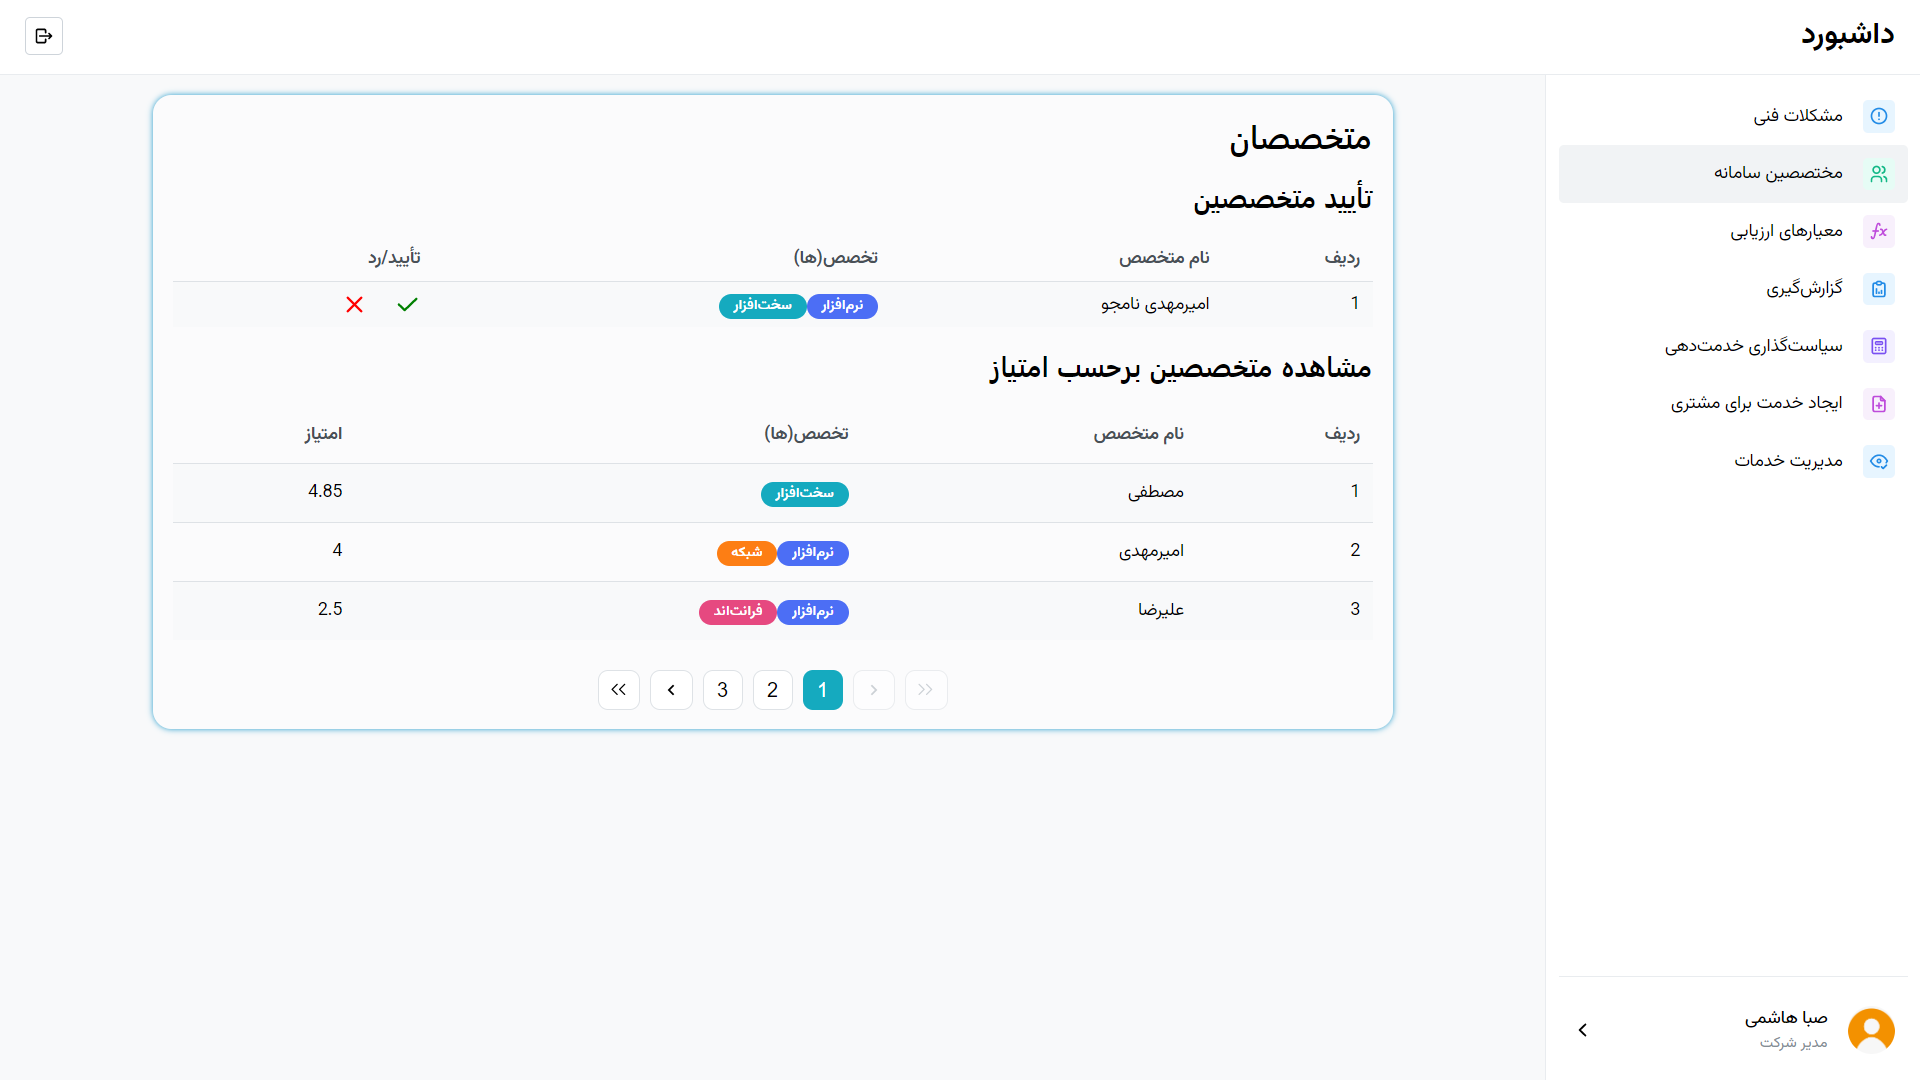
\includegraphics[width=\textwidth]{figs/initial-ui/mngr-specialists}
	\caption{امکان تأیید یا رد متخصص توسط مدیر فنی و مدیر شرکت}
	\label{mngr-specialists}
\end{figure}

\subsubsection{امکان لغو خدمت در هر مرحله}
این ویژگی (شماره 23) به مدیر فنی و مدیر شرکت این اجازه را می‌دهد که خدمات درخواست‌شده‌ی مشتریان را در هر مرحله‌ای لغو کنند. این ویژگی در شکل
\ref{cancel-service}
نمایش داده شده است.

\begin{figure}[h]
	\centering
	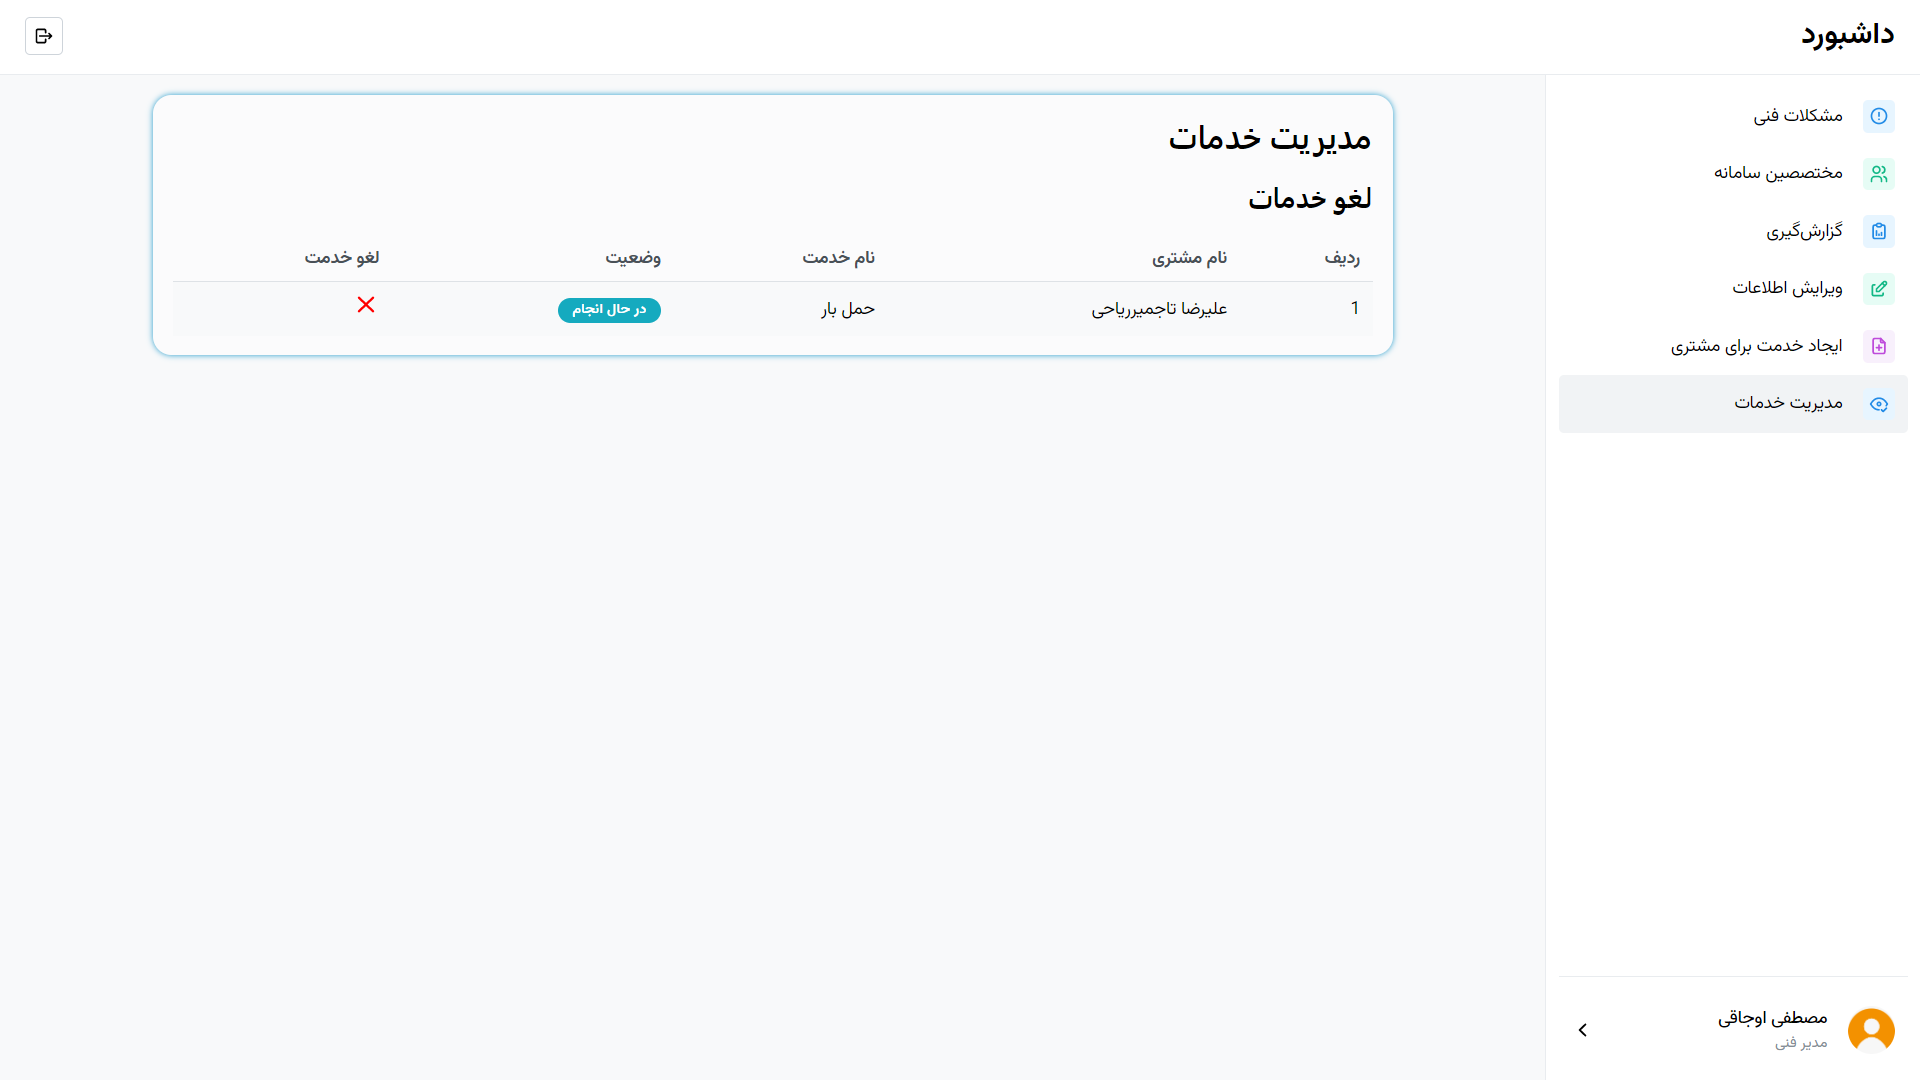
\includegraphics[width=\textwidth]{figs/initial-ui/cancel-service}
	\caption{امکان تأیید یا رد متخصص توسط مدیر فنی و مدیر شرکت}
	\label{cancel-service}
\end{figure}









